\documentclass[a4paper,11pt]{article}
\usepackage[margin=20mm]{geometry}
\usepackage{amsmath,amssymb,graphicx,booktabs,array,float,hyperref}
\hypersetup{hidelinks}
\setlength{\parindent}{0pt}
\setlength{\parskip}{5pt}
\renewcommand{\arraystretch}{1.14}
\setlength{\tabcolsep}{4pt}
\begin{document}
\thispagestyle{empty}
\begin{center}{\Large\bfseries Beihang University\\School of Mathematical Sciences\\Laboratory Report}\end{center}
{\small Detailed derivations, results and analysis continue on the following pages.}\par
\vspace{3mm}
\begin{tabular}{|p{.22\linewidth}|p{.22\linewidth}|p{.22\linewidth}|p{.22\linewidth}|}\hline
\multicolumn{2}{|p{.47\linewidth}|}{Course: Numerical Analysis Computer Laboratory} & \multicolumn{2}{p{.43\linewidth}|}{Best Square Approximation Homework}\\\hline
\multicolumn{4}{|l|}{Experiment type: Demonstration [ ] Verification [ ] Comprehensive [ ] Design [ ]}\\\hline
Class: 230116 & \multicolumn{2}{l|}{Name: yule yang} & Student ID: 23376268\\\hline
Lab date: 2026.10.17 & \multicolumn{2}{l|}{Instructor:} & Grade:\\\hline

\multicolumn{4}{|p{.95\linewidth}|}{\textbf{Experimental environment}\par Analytic derivations checked with Python, NumPy and 160 point Gauss Legendre quadrature; Matplotlib for figures. AI assistance: Codex.\par\vspace{4mm}}\\\hline
\multicolumn{4}{|p{.95\linewidth}|}{\textbf{Objectives and content}\par Answer every subquestion in Problems 1 through 6: Gram matrix formulation, the best line for x squared, orthonormal projection, Legendre approximation, weighted approximation, and the best quadratic for sine.\par\vspace{4mm}}\\\hline
\multicolumn{4}{|p{.95\linewidth}|}{\textbf{Procedure and results}\par All six problems are solved with derivations. The best line for x squared is x - 1/6; x cubed projects to 3x/5 in degree at most two; sine projects to 3x/pi. Independent quadrature checks all numerical identities.\par\vspace{4mm}}\\\hline
\multicolumn{4}{|p{.95\linewidth}|}{\textbf{Analysis and conclusions}\par The residual is orthogonal to the approximation space. Positive Gram matrices imply unique coefficients. Orthogonal bases simplify computation, symmetry eliminates incompatible parity terms, and weighted inner products change which errors receive emphasis.\par\vspace{4mm}}\\\hline
\end{tabular}
\clearpage
\section*{Problem 1 Gram matrix formulation}
Assume a < b, f belongs to L2[a,b], and the real basis functions phi0 through phin are independent as elements of that inner product space. For continuous functions, ordinary linear independence implies this condition: a nonzero continuous combination is nonzero on an interval of positive measure. For arbitrary discontinuous representatives, independence only at isolated points would not suffice.

\[p=\sum_{j=0}^{n}c_j\phi_j,\qquad E(c)=\left\|f-\sum_{j=0}^{n}c_j\phi_j\right\|_2^2.\]
\[E(c)=\langle f,f\rangle-2\sum_jc_j\langle f,\phi_j\rangle+\sum_i\sum_jc_ic_j\langle\phi_i,\phi_j\rangle.\]
Differentiate with respect to each coefficient. At a minimum all partial derivatives vanish, producing n + 1 normal equations. Define the Gram entries and right hand side by the following integrals.

\[G_{ij}=\langle\phi_j,\phi_i\rangle=\int_a^b\phi_i(x)\phi_j(x)\,dx,\qquad b_i=\langle f,\phi_i\rangle.\]
\[\frac{\partial E}{\partial c_i}=2\sum_jG_{ij}c_j-2b_i=0,\qquad Gc=b.\]
Symmetry follows because multiplication of real functions commutes. For any nonzero coefficient vector z, independence implies its linear combination is nonzero in L2. Hence its squared norm is strictly positive:

\[z^TGz=\int_a^b\left(\sum_jz_j\phi_j(x)\right)^2dx>0.\]
Thus G is symmetric positive definite and invertible. The normal system has exactly one coefficient vector. Moreover the Hessian of E is 2G, so E is strictly convex and this stationary point is the unique global minimum. Equivalently, if p star is the solution, residual orthogonality gives the Pythagorean identity below for every q in the approximation space.

\[\|f-q\|_2^2=\|f-p_*\|_2^2+\|p_*-q\|_2^2.\]
The extra term is nonnegative and vanishes only when q equals p star in L2. For continuous functions, equality in L2 also gives pointwise equality. This proves existence and uniqueness of both the function and its coefficient representation under the stated independence assumption.

\clearpage
\section*{Problem 2 Best linear approximation on the unit interval}
Write p(x) = c0 + c1 x. The least squares functional and its explicit expansion are:

\[E(c_0,c_1)=\int_0^1(x^2-c_0-c_1x)^2dx.\]
\[E=\frac15-\frac{2c_0}{3}-\frac{c_1}{2}+c_0^2+c_0c_1+\frac{c_1^2}{3}.\]
Setting the two partial derivatives to zero is equivalent to requiring the residual to be orthogonal to 1 and x. The moment system is:

\[\begin{pmatrix}1&1/2\\1/2&1/3\end{pmatrix}\begin{pmatrix}c_0\\c_1\end{pmatrix}=\begin{pmatrix}1/3\\1/4\end{pmatrix}.\]
From the first equation c0 = 1/3 - c1/2. Substitution into the second gives c1/12 = 1/12; consequently c1 = 1 and c0 = -1/6.

\[p_*(x)=x-\frac16,\qquad r(x)=x^2-x+\frac16.\]
\[\|r\|_2^2=\int_0^1\left(x^2-x+\frac16\right)^2dx=\frac1{180}.\]
For a second error calculation, the normal equations imply the inner product of f with its projection equals the squared norm of the projection. The inner product is (-1/6)(1/3) + 1/4 = 7/36, while the norm squared of f is 1/5.

\[\|f-p_*\|_2^2=\frac15-\frac7{36}=\frac1{180}\approx0.005555555556.\]
The Gram determinant is 1/12, so the stationary point is uniquely minimizing. The approximation is not constrained to interpolate endpoints. Its total L2 norm error is the square root of 1/180, whereas the requested squared error is 1/180.

\clearpage
\section*{Problem 3 Orthonormal projection formula}
Let psi0 through psin be an orthonormal basis for Vn. In these coordinates the Gram matrix is the identity. Therefore the normal equations directly give each coefficient as the inner product of f with its basis function.

\[\alpha_k=\langle f,\psi_k\rangle,\qquad p_n^*=\sum_{k=0}^{n}\alpha_k\psi_k.\]
Indeed, for every j the inner product of f minus this sum with psij is alpha j minus alpha j, which equals zero. Every q in Vn is a linear combination of the basis, so the residual is orthogonal to all of Vn and the projection is optimal by the Pythagorean identity from Problem 1.

\[\|p_n^*\|_2^2=\sum_{k=0}^{n}|\alpha_k|^2,\qquad \langle f-p_n^*,p_n^*\rangle=0.\]
\[\|f-p_n^*\|_2^2=\|f\|_2^2-\sum_{k=0}^{n}|\langle f,\psi_k\rangle|^2.\]
The absolute value squared notation also works in a complex Hilbert space when the inner product uses conjugation and the corresponding consistent coefficient convention. For the real function spaces in this assignment it is simply an ordinary coefficient square.

\subsection*{Enlarging the approximation space}
\[E_{n+1}=E_n-|\langle f,\psi_{n+1}\rangle|^2\leq E_n.\]
Adding one orthonormal direction removes the squared energy of that new component. Error is unchanged exactly when the new inner product is zero; otherwise it strictly decreases. The same monotonicity holds for any nested approximation spaces because every old candidate remains admissible, even if the supplied bases are not orthonormal.

This is a finite projection identity; no completeness assumption about an infinite basis is needed. Taking an infinite limit would require additional hypotheses. Since the residual norm is nonnegative, the coefficient energy sum is bounded above by the norm squared of f, giving the finite form of Bessel inequality.

\clearpage
\section*{Problem 4 Legendre polynomial approximation}
The basis P0 = 1, P1 = x and P2 = (3x squared - 1)/2 is orthogonal on [-1,1]. It is not orthonormal, so each inner product must be divided by the appropriate squared norm.

\[p_2(x)=a_0P_0(x)+a_1P_1(x)+a_2P_2(x),\qquad a_j=\frac{\langle x^3,P_j\rangle}{\langle P_j,P_j\rangle}.\]
\[\langle x^3,P_0\rangle=\int_{-1}^1x^3dx=0,\qquad \langle x^3,P_1\rangle=\int_{-1}^1x^4dx=\frac25.\]
\[\langle x^3,P_2\rangle=\frac12\int_{-1}^1(3x^5-x^3)dx=0.\]
\[(a_0,a_1,a_2)=\left(0,\frac{2/5}{2/3},0\right)=\left(0,\frac35,0\right).\]
\[p_2=0P_0+\frac35P_1+0P_2=\frac35x.\]
The P2 coefficient vanishes because x cubed is odd and P2 is even; their product is odd on a symmetric interval. The same argument removes P0. A degree at most two approximation can therefore have degree one. Including an even quadratic term cannot help approximate an odd target under this symmetric unweighted inner product.

\subsection*{Error and an independent analytic check}
\[\|x^3-p_2\|_2^2=\frac27-\frac{(2/5)^2}{2/3}=\frac8{175}\approx0.04571428571.\]
\[P_3=\frac12(5x^3-3x),\qquad x^3=\frac35P_1+\frac25P_3.\]
The omitted P3 component is orthogonal to every polynomial of degree at most two. Its squared norm is (2/5) squared times 2/7 = 8/175, confirming both the coefficient and the residual energy.

\clearpage
\section*{Problem 5 Weighted best square approximation}
Let w be continuous and strictly positive on the compact interval [a,b]. It has a positive minimum and a finite maximum, so it defines an inner product equivalent to the unweighted L2 inner product. The weighted best approximation minimizes:

\[p_w^*=\arg\min_{p\in V_n}\|f-p\|_w^2,\qquad \|g\|_w^2=\int_a^bg(x)^2w(x)dx.\]
For any direction q in Vn, differentiate the weighted squared error along p star plus epsilon q. At epsilon = 0 the derivative must vanish, giving the condition for all q:

\[0=\left.\frac{d}{d\varepsilon}\|f-p_w^*-\varepsilon q\|_w^2\right|_{\varepsilon=0}=-2\langle f-p_w^*,q\rangle_w.\]
\[\langle f-p_w^*,q\rangle_w=0\quad\text{for every }q\in V_n.\]
\[G^{(w)}_{ij}=\int_a^b\phi_i\phi_jw\,dx,\qquad b^{(w)}_i=\int_a^bf\phi_iw\,dx,\qquad G^{(w)}c=b^{(w)}.\]
For a nonzero vector z, its weighted Gram quadratic form is the integral of the squared nonzero basis combination times the positive weight, hence is strictly positive. Thus the weighted solution is unique. Weighted residual orthogonality is also sufficient for optimality, by the weighted Pythagorean identity.

\subsection*{Effect of the weight and a concrete example}
Larger weights impose a greater penalty on errors in those regions. Multiplying the entire weight by a positive constant leaves the optimizer unchanged. In instrument calibration with known spatially varying uncertainty, a weight proportional to inverse error variance can emphasize more reliable readings. This is a modeling choice, not a claim of measured uncertainty here.

For an explicit continuous example, fit x squared by a line on [0,1] with w(x) = 1 + x. The system and solution are:

\[\begin{pmatrix}3/2&5/6\\5/6&7/12\end{pmatrix}\begin{pmatrix}c_0\\c_1\end{pmatrix}=\begin{pmatrix}7/12\\9/20\end{pmatrix},\qquad p_w^*(x)=-\frac5{26}+\frac{68}{65}x.\]
This weight places progressively more emphasis near x = 1. The resulting line differs from the unweighted x - 1/6 and is checked by weighted residual orthogonality.

\clearpage
\section*{Problem 6 Best quadratic approximation to sine}
For f(x) = sin(pi x), use basis 1, x, x squared on [-1,1]. The Gram entry is the integral of x to the power i + j. Odd moments vanish; even moments are 2/(i+j+1). The constant and quadratic right hand sides vanish by parity.

\[\int_{-1}^1x\sin(\pi x)dx=2\left[-\frac{x\cos(\pi x)}\pi+\frac{\sin(\pi x)}{\pi^2}\right]_0^1=\frac2\pi.\]
\[\begin{pmatrix}2&0&2/3\\0&2/3&0\\2/3&0&2/5\end{pmatrix}\begin{pmatrix}c_0\\c_1\\c_2\end{pmatrix}=\begin{pmatrix}0\\2/\pi\\0\end{pmatrix}.\]
The middle equation gives c1 = 3/pi. The even coefficient block is invertible, with determinant 16/45, so c0 = c2 = 0. An odd target has no even projection component under this symmetric inner product.

\[p_2(x)=\frac3\pi x,\qquad \|f-p_2\|_2^2=1-\frac6{\pi^2}\approx0.3920728981.\]
\subsection*{Comparison with the Taylor polynomial}
\[\sin(\pi x)=\pi x-\frac{\pi^3x^3}{6}+\cdots,\qquad T_2(x)=\pi x.\]
\[\|f-ax\|_2^2=1-\frac{4a}{\pi}+\frac{2a^2}{3}.\]
\[\|f-T_2\|_2^2=\frac{2\pi^2}{3}-3\approx3.579736267.\]
Taylor matches derivatives at zero and is locally accurate; the best square approximation balances error across the whole interval. Their slopes differ because they optimize different criteria. The requested degree two Taylor polynomial is pi x, not the cubic truncation. The projection has substantially lower integrated squared error, while Taylor has the correct derivative at the origin.

\clearpage
\section*{Numerical verification and reproducibility}
All 16 of 16 independent numerical checks pass. A 160 node Gauss Legendre quadrature rule verifies Gram matrices, coefficients, orthogonality and squared errors. Polynomial integrals through degree six are within the rule's exactness range in exact arithmetic; the sine integrals provide a smooth nonpolynomial check.

{\small\begin{tabular}{p{0.3153333333333333\linewidth}p{0.3153333333333333\linewidth}p{0.3153333333333333\linewidth}}\toprule
Problem & Quantity & Verified value\\\midrule
2 & Squared error & 0.005555555556\\
4 & Squared error & 0.045714285714\\
5 & Weighted coefficients & -5/26 and 68/65\\
6 & Projection squared error & 0.392072898146\\
6 & Taylor squared error & 3.579736267393\\
\bottomrule\end{tabular}}\par
\begin{figure}[H]\centering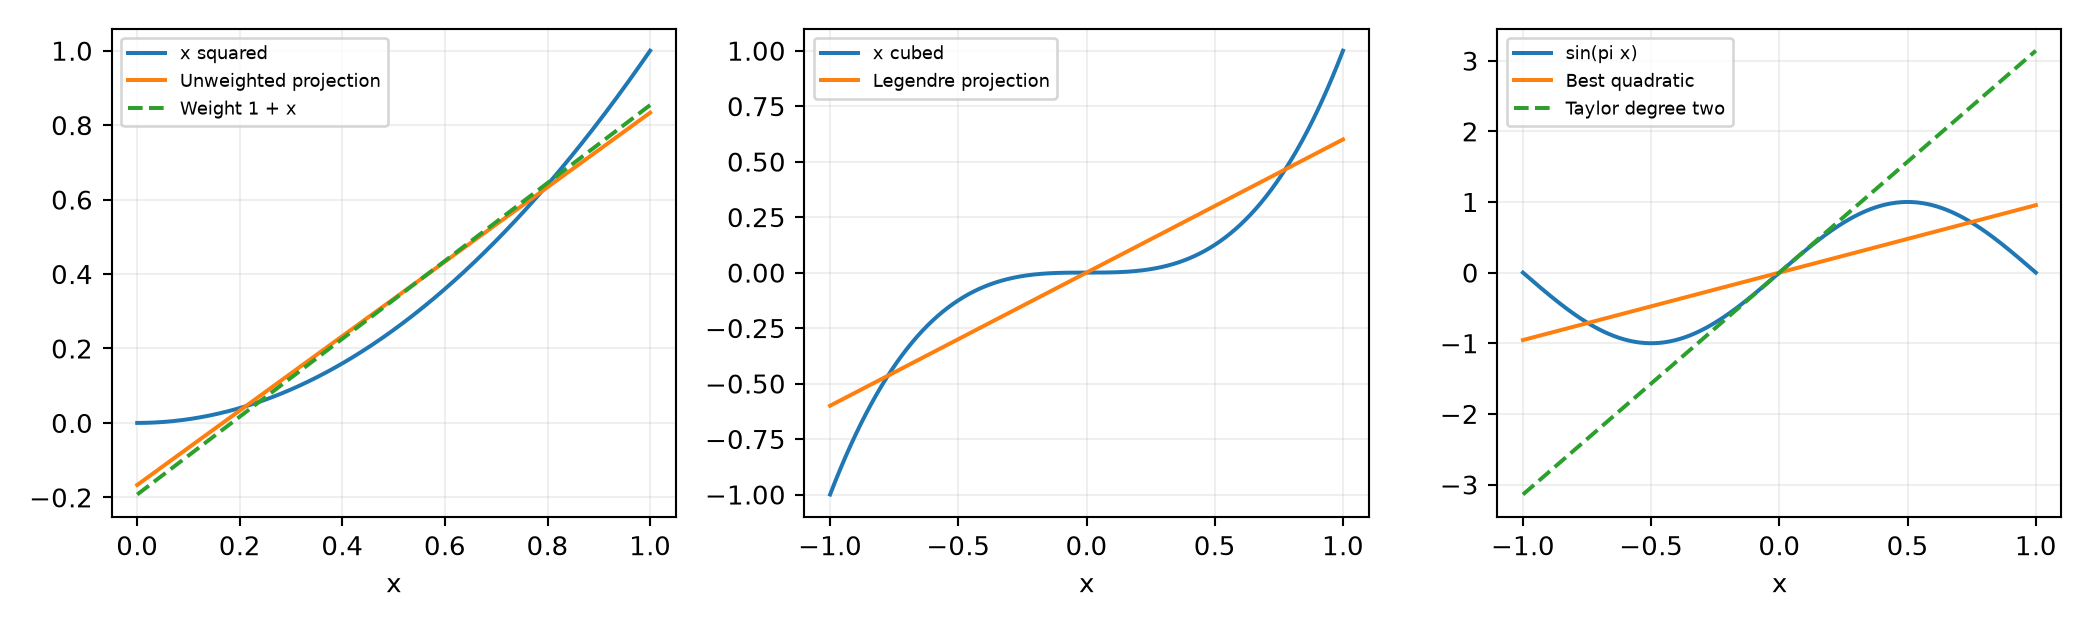
\includegraphics[width=\linewidth,height=57.15mm,keepaspectratio]{figures/projections.png}\caption{Computed functions and their analytic projections. The first panel also illustrates a strictly positive nonconstant weight.}\end{figure}
The code is a verification of the analytic derivations, not a replacement for them. It records all quadrature nodes and weights, package versions, computed systems and verification outcomes. No random data or external observations are needed.

From the package root, run python reproduce.py to regenerate numerical results, verification, figures, report content, the LaTeX PDF and the editable Word document. See README.md for the individual commands and directory layout. The final PDF is compiled from LaTeX before Word generation; the Word document uses native editable Office equations.

Source: the supplied four page Best Square Approximation Homework Assignment. Problems 1 through 6 and all of their numbered subquestions are answered in the preceding sections. The optional weighted line example supplements Problem 5; it is labeled as an illustration rather than an additional requirement.

\end{document}